\clearpage

\section{Theoretical Analysis}
\label{sec:analysis}

In this part we will discuss the theoretical analysis of the circuit shown in \ref{fig:circuito}.
In order to do that we will have to do both DC and AC analysis.

For the DC analysis, we can analyse both stages separatly, so we can do the following:
\begin{itemize}
    \item Find the DC equivalent circuit by replacing all capacitors by open circuits;
    \item Find Q-point (steady-state voltage or current at a specified terminal of an active device with no input signal applied) from DC equivalent circuit by using appropriate transistor model.
\end{itemize}

For the AC analysis:
\begin{itemize}
    \item Find AC equivalent circuit by replacing all capacitors by short circuits and DC voltage sources by ground connections;
    \item Replace transistor by its hybrid $\Pi$ model;
    \item Use small-signal AC equivalent to analyze AC characteristics of amplifier.
\end{itemize}

In the end, we just need to combine the end results of DC and AC analysis to yield the total voltages and currents in the network.

With this being said, let's start by the DC analysis of the gain stage and output stage, which can be done separately.

\subsection{DC analysis}
\subsubsection{Gain stage}
Replacing all capacitors with open circuits leaves us with the circuit shown in figure \ref{fig:DC analysis}.

Replacing all connections to the transistor with their Thévenin equivalents gives the circuit presentend in figure
\ref{fig:Thevenin}, and applying KVL to the transistor yields the following expression: 

\begin{equation}
  V_{eq}-I_{B}R_{eq}-V_{BE}-I_{E}R_{E}=0
\end{equation}

\begin{multicols}{2}

  \begin{figure}[H]
  \begin{center}
   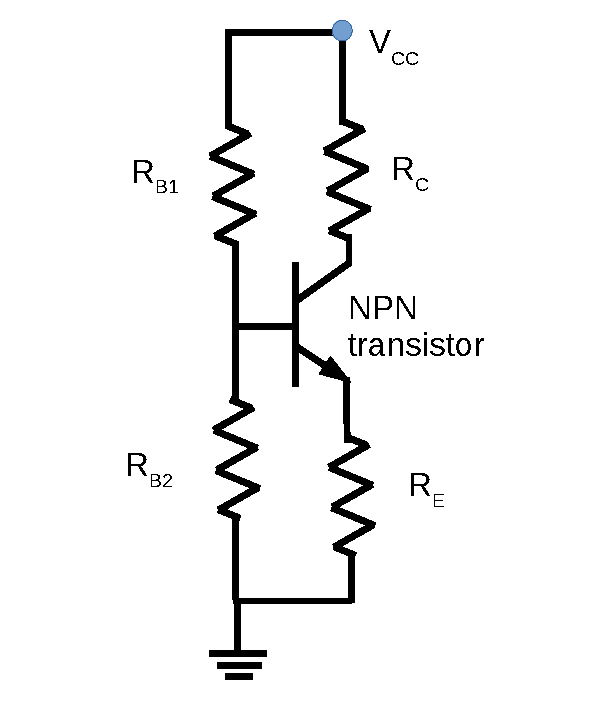
\includegraphics[width=6cm]{lab4_DC1.pdf}
  \caption{Gain stage OP computation.}
  \label{fig:DC analysis}
  \end{center}
  \end{figure}
  
  
  \begin{figure}[H]
  \begin{center}
   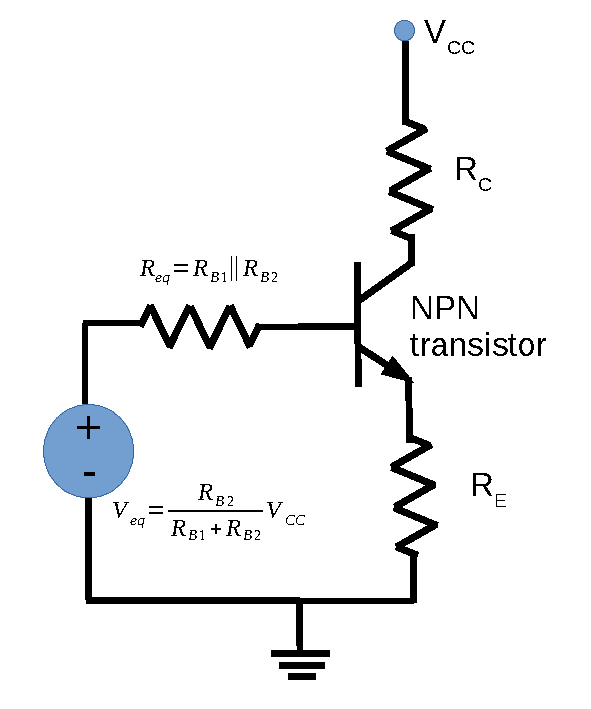
\includegraphics[width=6cm]{lab4_DC1_TH.pdf}
  \caption{Thévenin equivalent.}
  \label{fig:Thevenin}
  \end{center}
  \end{figure}
\end{multicols}

Applying KCL to the transistor:
\begin{equation}
    I_{E}=I_{B}+I_{C}
\end{equation}
Because $I_{C}=\beta \times I_{B}$:
\begin{equation}
    I_{E}=I_{B}\left( 1+\beta \right)
\end{equation}
Substituting for $I_{E}$ in the loop equation:
\begin{equation}
    V_{eq}-I_{B}Req-V_{BE}-I_{B}\left( 1+\beta \right) R_{E}=0
\end{equation}
We can assume $V_{BE}\approx 0.7V$ (the usual potencial barrier).
With further development of these equations, we can get all the voltages and current values we need, mainly the current through the collector, 
to use in the AC analysis, and the voltage drop between collector and emitter, to check if the transistor is in the forward active region and to compare the 
theoretical with the simulation results. 
These results are shown in table \ref{tab:op1_tab}.

\begin{table}[h]
    \centering
    \begin{tabular}{|l|r|}
      \hline
      {\bf Name} & {\bf Value [A or V]} \\ \hline
      \input{../mat/op1_tab.tex}
    \end{tabular}
    \caption{Current through collector and the voltage drop between collector and emitter.}
    \label{tab:op1_tab}
  \end{table}


As we can see $V_{CE} > V_{BE}=V_{BE_{ON}}$, so we know that the transistor is in the forward active region.

\subsubsection{Output stage}
For the Output stage, the analysed circuit is shown in figure \ref{fig:Thevenin2}.

\begin{figure}[H]
  \begin{center}
   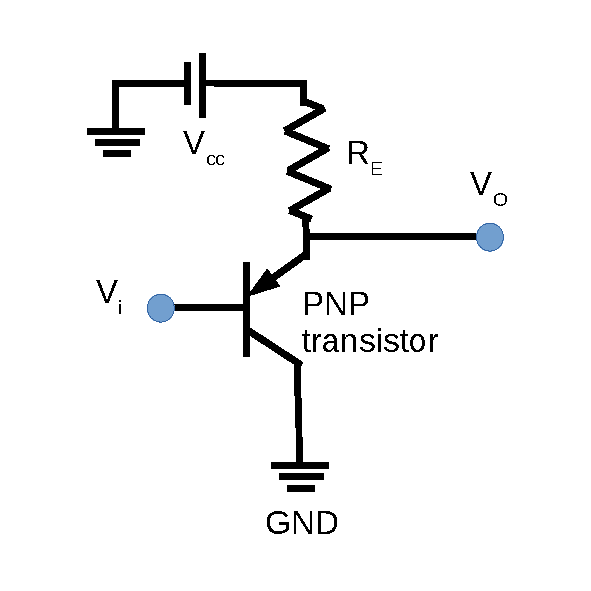
\includegraphics[width=10cm]{lab4_DC2.pdf}
  \caption{Output stage (DC analysis).}
  \label{fig:Thevenin2}
  \end{center}
  \end{figure}

We assume that $V_{EB}\approx 0.7V$.
Applying KVL to all meshes and knowing that the voltage $V_{I}$ is equal to the output of the gain stage we get:
\begin{equation}
    I_{E}=\frac{V_{CC}-V_{EB}-V_{I}}{R_{E}}
\end{equation}
\begin{equation}
    V_{O}=V_{cc}-R_{E}I_{E}
\end{equation}
\begin{equation}
    V_{O}=V_{I}+V_{BE}
\end{equation}

Once again, with further development of these equations, we can get the same currents and voltages as for the gain stage, as shown in table \ref{tab:op2_tab}.

\begin{table}[h]
    \centering
    \begin{tabular}{|l|r|}
      \hline
      {\bf Name} & {\bf Value [A or V]} \\ \hline
      \input{../mat/op2_tab.tex}
    \end{tabular}
    \caption{Current through collector and the voltage drop between emitter and collector.}
    \label{tab:op2_tab}
  \end{table}

As we can see $V_{EC} > V_{EB}=V_{EB_{ON}}$, so we know that the transistor is in the forward active region.

\subsection{AC analysis}
With the operating point analysis done, we can now replace the capacitors with short circuits and start the AC analysis, using incremental analysis. 
In this subsection, we have only considered the incremental analysis for medium frequencies, and that is why it is possible to replace the capacitors with short circuits. 
In addition, all the DC-only sources can be replaced with short circuits, too, and the transistors can be replaced with the corresponding incremental model. 
We first studied the gain stage and the output stage independently.

\subsubsection{Gain stage}
The resulting circuit can be simplified to:

\begin{figure}[h] \centering
    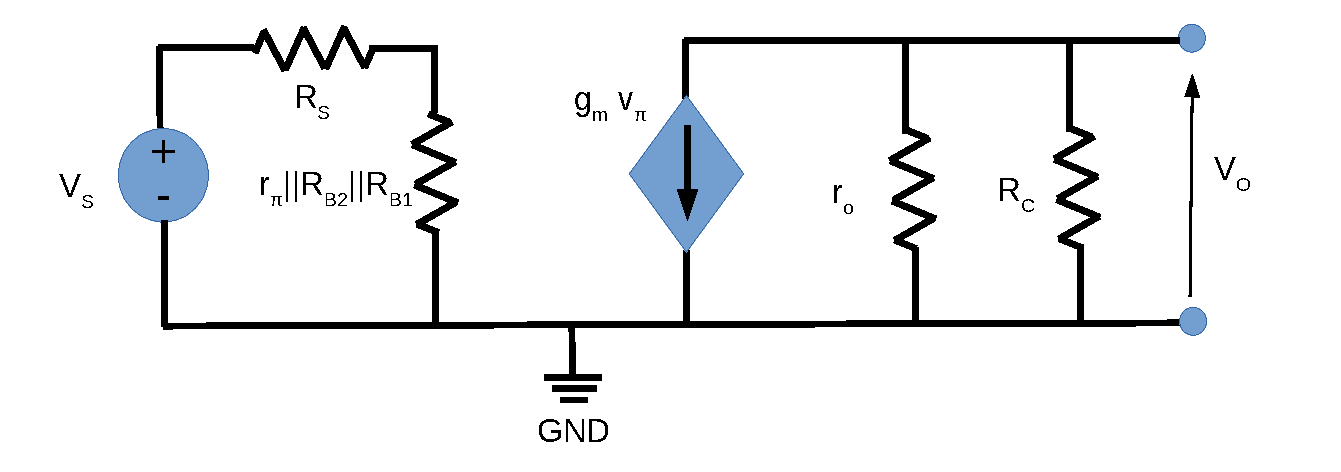
\includegraphics[width=17cm]{lab4_AC1.pdf}
    \caption{Gain stage AC analysis - incremental circuit.}
    \label{fig:AC1 analysis}
\end{figure}

\clearpage

As we derived in the theotherical classes we have that:

\begin{equation}
    \begin{cases}
        \dfrac{v_{o}}{v_{i}}=-g_{m}\left( R_{c}\| R_{0}\right) v_{\pi } \\
        v_{\pi }=\dfrac{r_{\pi }\left\| R_{B1}\right\| R_{B2}}{R_{s}+r_{\pi }\left\| R_{B1}\right\| R_{B2}}
    \end{cases}
\end{equation}
\begin{equation}
    \Rightarrow \dfrac{v_{o}}{v_{i}}=-g_{m}\left( R_{c}\| R_{0}\right) \dfrac{r_{\pi }\left\| R_{B1}\right\| R_{B2}}{R_{s}+r_{\pi }\left\| R_{B1}\right\| R_{B2}}
\end{equation}
For the input and output impendances we have:
\begin{equation}
    \begin{cases}
        Z_{I}=R_{B1}\left\| R_{B2}\right\| r_{\pi } \\
        Z_{0}= R_{c}\| r_{O}
    \end{cases}
\end{equation}

The results are presented in table \ref{tab:stage1_tab}.
\begin{table}[h]
    \centering
    \begin{tabular}{|l|r|}
      \hline
      {\bf Name} & {\bf Value [- or $\Omega$]} \\ \hline
      \input{../mat/Stage1_tab.tex}
    \end{tabular}
    \caption{Gain and impedances.}
    \label{tab:stage1_tab}
  \end{table}

\subsubsection{Output stage}
The resulting circuit can be simplified to:

\begin{figure}[H]
    \begin{center}
     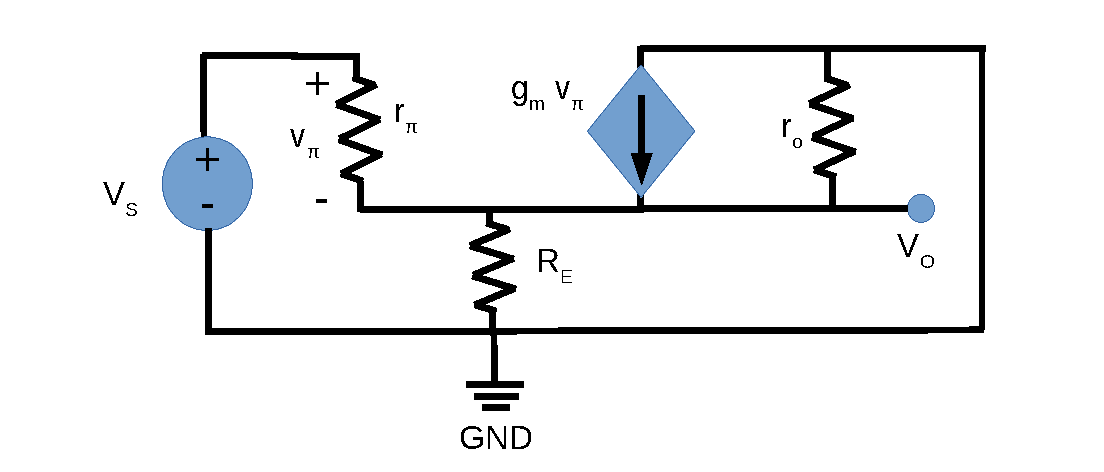
\includegraphics[width=15cm]{lab4_AC2.pdf}
    \caption{Output stage AC analysis - incremental circuit.}
    \label{fig:AC2 analysis}
    \end{center}
  \end{figure}

Relative to the output stage we got:
\begin{equation}
    \dfrac{v_{0}}{v_{i}}=\dfrac{g_{m}}{g_{\pi }+g_{E}+g_{o}+g_{m}}
\end{equation}
\begin{equation}
    Z_{I}=\dfrac{g_{\pi }+g_{E}+g_{o}+g_{m}}{g_{\pi} \left( g_{\pi} +g_{E}+g_{o}\right) }
\end{equation}
\begin{equation}
    Z_{o}=\dfrac{1}{g_{\pi }+g_{E}+g_{o}+g_{m}}
\end{equation}

\clearpage

The results are presented in table \ref{tab:stage2_tab}.
\begin{table}[h]
    \centering
    \begin{tabular}{|l|r|}
      \hline
      {\bf Name} & {\bf Value [- or $\Omega$]} \\ \hline
      \input{../mat/Stage2_tab.tex}
    \end{tabular}
    \caption{Gain and impedances.}
    \label{tab:stage2_tab}
\end{table}

As we can see the gain stage output impedance and the output stage input impedance are quite compatible
and that garantees that they can be connected without significant signal loss.

\subsection{Frequency response}

Now we will calculate the frequency response $\dfrac{V_{o}(f)}{V_{I}(f)}$. For this, we need the total incremental circuit, as shown below:

\begin{figure}[H] \centering
    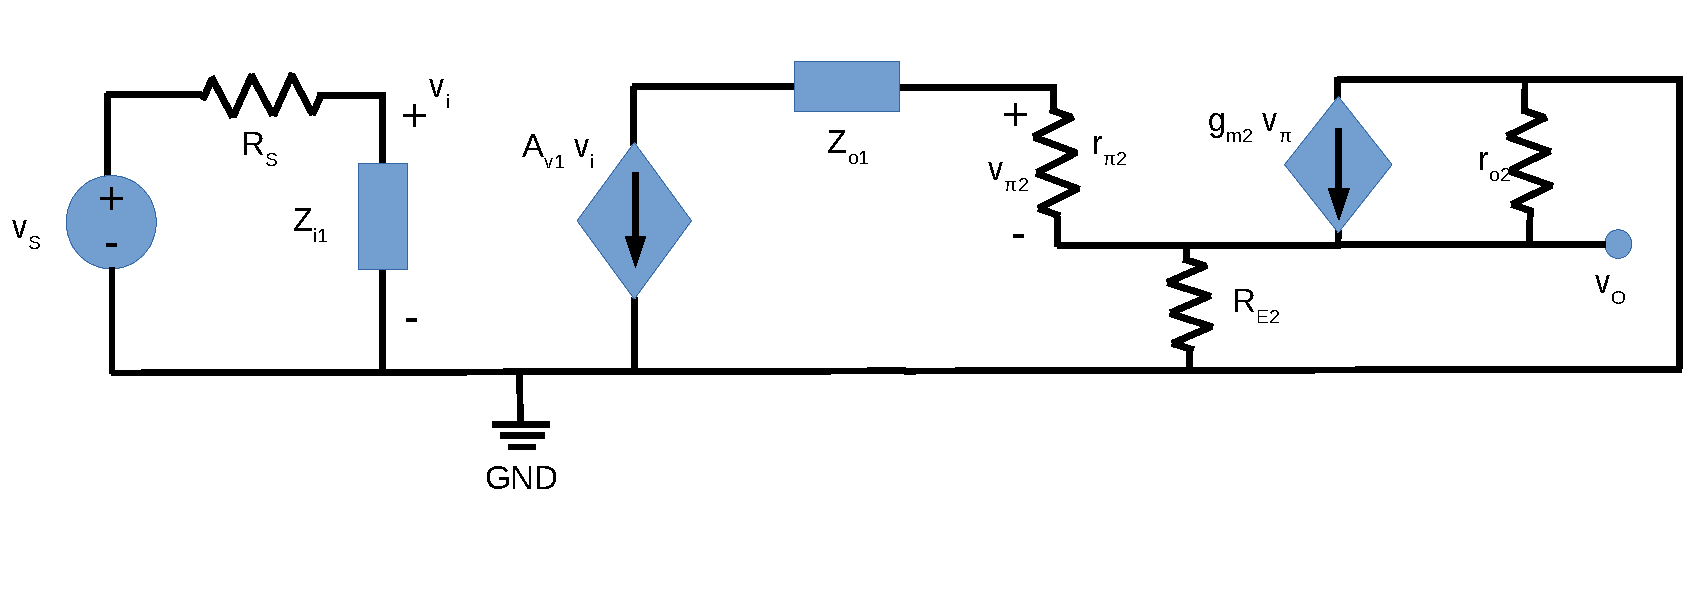
\includegraphics[scale=0.55]{lab4_AC_Total.pdf}
    \caption{Complete circuit.}
    \label{fig:CompleteCircuit}
\end{figure}
 
The gain was only calculated for medium frequencies, so we end up considering the frequency response as a 
constant value (equivalent to saying that the cut off frequencies are 0 and $\infty$). The gain was calculated using the following expression:

\begin{equation}
    \frac{v{o}}{v{i}}=\frac{\frac{1}{r_{\pi_{2}}+Z_{o1}}+\frac{g_{m2}r_{\pi2}}{r_{\pi_{2}}+Z_{o1}}}{\frac{1}{r_{\pi_{2}}+Z_{o1}}+\frac{1}{R_{E2}}+\frac{1}{r_{o2}}+\frac{g_{m2}r_{\pi2}}{r_{\pi_{2}}+Z_{o1}}}A_{v1}
\end{equation}

where $A_{v1}$ is the gained obtained for the gain stage.
 In the following graphic we present the frequency response, ranging from $10 Hz$ to $100 Mhz$, in logarithmic scale and with $10$ points per decade.

 \begin{figure}[H] \centering
    \includegraphics[scale=0.80]{Octave_t4.pdf}
    \caption{Theoretical gain.}
    \label{fig:Octave_t4}
\end{figure}

\section{Comparison}

As one may notice, there are a few differences when comparing \textit{Ngspice}'s and \textit{Octave}'s results.
But this is somewhat normal since the models used in the theoretical analysis are approximations of non linear components that are the transistors.
Moreover, the Hybrid $\Pi$ model used was not the full one, so we did not take into account the Miller effect and complete Early Effect
that occurs in this type of network. Despite this, the results are quite satisfactory.
